\chapquote{"Video killed the radio star."}{The Buggles}{1979}

\section{Introduction}

\section{The Far-Infrared/Radio Correlation}

For samples of star forming galaxies in the local and high redshift universe there is a well observed correlation between the far-infrared and radio emission (e.g. \citealt{Dickey_1984}; \citealt{deJong_1985}; \citealt{Helou_1985}; \citealt{Condon_1992}; \citealt{Barger_2000}; \citealt{Yun_2001}; \citealt{Garrett_2002}; \citealt{Appleton_2004}; \citealt{Ibar_2008}; \citealt{Seymour_2009}; \citealt{Sargent_2010}), that remains nearly linear over multiple orders of magnitude in far-infrared luminosity ($10^{9} \lesssim L_{\textrm{FIR}} [L_{\odot}] \lesssim 10^{12.5}$). The small scatter in this relation is often attributed to the "calorimeter model" (\citealt{Voelk_1989}; \citealt{Lisenfeld_1996}; \citealt{Lacki_2010}), which ascribes the far-infrared and radio emission to common stellar sources. In this model, galaxies are assumed to be opaque to UV light from massive OB stars which gets absorbed by the dust in the ISM and reradiated in the far-infrared. Observations in the far-infrared and sub-mm are thus sensitive to the cold dust that reradiates the energy from young stars. These stars quickly come to the end of their lives, exploding as Type II supernovae producing cosmic ray electrons and positrons. Most of their energy gets radiated in the radio as synchrotron radiation when interacting with the magnetic fields of the supernova remnant. The radio continuum is therefore a tracer of recent, obscured star formation.

Despite a higher scatter for high redshift SMGs than with local samples, the far-infrared/radio correlation (FIRC) still holds at increasing redshift (\citealt{Ivison_2010a}; \citealt{Ivison_2010b}). {\color{red}Small description on evolution of FIRC with redshift.}

The appearance of a correlation at all redshifts and luminosities has facilitated studies that use the radio emission as an unbiased tracer of obscured star formation in dusty galaxies (\citealt{Kennicutt_2012}). By making use of the tight correlation (as well as the benefits we outline in the following section), we can identify counterparts to single dish sub-mm observations with large beams with greater confidence than we would expect from the optical or near-infrared. This allows for better characterization of the properties of SMGs and allows us to study the cosmic star formation history to higher redshifts (\citealt{Madau_2014}; \citealt{Delhaize_2017}; \citealt{Novak_2017}).

\section{Identifying Multiwavelength Counterparts to SMGs via Radio IDs}

As illustrated in Chapter \ref{chapter:Data_Release_3}, SMGs that are detected with single dish sub-mm telescopes with low angular resolution will likely include multiple galaxies in the optical or near-infrared within the beam width. This is a particular problem for \textit{Herschel} where even the smallest beam size at 250\,\micron\ has a FWHM of $\sim$ 18 arcsec. The possibility of tightly clustered SMGs (\citealt{Blain_2004}) and with a higher surface density of optical counterparts, deciding unambiguously on the source of the sub-mm emission is difficult. This is further compounded by their intrinsic faintness due to the dust obscuration. The optimal way to overcome the problem of poor resolution is to follow up with millimetric or longer wavelength interferometric observations. In the following sections we detail a method for identifying radio counterparts to \textit{Herschel} sources in order to secure unambiguous multiwavelength counterparts to our sub-mm galaxies. The following is a list of benefits of using the radio emission to select counterparts throughout the electromagnetic spectrum.

\begin{enumerate}
    \item Star forming galaxies produce a lot of synchrotron emission. This allows us to take advantage of the FIRC to locate the galaxy emitting radiation in the far-IR. Compared to searches in other wavelengths, such as using the Likelihood Ratio to identify optical counterparts, the search for identifications is not solely motivated by their position and brightness, but also by the physical link between the two objects due to their common source.
    \item Even when considering the deepest radio maps, the low surface density of radio sources means that the probability of chance positoinal coincidences with a sub-mm source is relatively unlikely. As a result, we can have a reasonable confidence in some association between objects when we do observe radio sources in close proximity to the sub-mm position (\citealt{Ivison_2002}; \citealt{Borys_2004}). In most cases (as we shall validate in this study), radio sources are sufficiently rare that finding an object within the positional uncertainty of the sub-mm beam almost always results in a robust identification.
    \item When a secure radio counterpart is identified, the positional accuracy ($\sim$ 1 arcsec for the Karl G. Jansky Very Large Array (VLA) at 1.4\,GHz and $\sim$ 0.75 arcsec at 3\,GHz) allows for a unambiguous identification with an optical or infrared galaxy counterpart. By locating these galaxies via the radio identification, we predict a low false identification rate of the SMG with the optical counterpart, allowing us to determine their morphologies, colours, magnitudes, stellar masses and more with greater confidence.
\end{enumerate}

While the radio emission from star-forming galaxies allows for secure identification of counterparts across the spectrum, it also has several drawbacks. The following is a list of disadvantages to using radio emission.

\begin{enumerate}
    \item Our understanding of the radio-selected SMG population is likely to be skewed by selection effects. The negative k-correction in the far-infrared arises due to the steep Rayleigh-Jeans part of the SED and allows for nearly equal detection of dusty galaxies at $z \sim 0.5$ as $z \sim 8$ for longer wavelengths where this effect is most pronounced (\citealt{Blain_2002}). The radio, however, suffers from a strong positive k-correction which causes a bias against high redshift galaxies ($z > 3$). This means that a substantial fraction of SMGs remain undetected in the radio due to the lack of sufficiently deep radio data. Despite this, we note that such deep radio data would produce a redshift distribution of SMGs much wider than we could obtain with the coverage of the SGP in the near-infrared (Chapter \ref{chapter:Data_Release_3}).
    \item Despite the benefit of the FIRC in locating radio galaxies in close proximity to SMGs, the correlation also causes a preference for the brightest SMGs, which may not be a representative sample of the full SMG population.
    \item Interferometry has been used to show that for sub-mm sources in which we observe multiple radio galaxies in close proximity, in $\sim$ 80\% of cases the sub-mm emission is associated from only one of the radio sources. This leads to an ambiguity as to the nature of some apparent multiple systems when interferometry is not available.
    \item Potentially the most pivotal drawback for the identification of sub-mm emitting galaxies, is the sky coverage from radio surveys. While we have large sky surveys in the sub-mm such as \textit{Herschel}-ATLAS, using radio data for large area sub-mm surveys is not yet practical. Future radio surveys such as the Square Kilometre Array (SKA) and recent wide-area surveys with the Low-Frequency Array (LOFAR) allow us to produce larger samples of SMGs to understand their stellar properties.
\end{enumerate}

Many studies (e.g. \citealt{Eales_2009}; \citealt{Dye_2009}) adopt a frequentist approach to searching for possible radio counterparts close to the submm position. This often involves using Monte Carlo simulations to estimate the probability that a given counterpart is located near the source by chance. The advantage of using a frequentist approach over a Bayesian method (Chapter \ref{chapter:Data_Release_3}) is that it does not require assumptions to be made on the form of the sub-mm positional errors, given that they are poorly known due to source confusion. As will be shown later, we can use the results of a frequentist approach to infer the distribution of positional errors. Despite this benefit, a frequentist approach would not have been appropriate for the VIKING counterparts we identified in the SGP because of their higher surface density {\color{red}[... Check my reasoning here ...]} 

\section{Identifying Radio IDs to \textit{Herschel} Sources in COSMOS}

In the following sections we identify radio counterparts to \textit{Herschel} detected sources in the Cosmic Evolution Survey (COSMOS). We applied the frequentist method of \citealt{Lilly_1999}, which differs from the Bayesian Likelihood Ratio method in that it searches for objects close to the sub-mm source and estimates the probability that each object is a chance alignment, rather than estimating the probability the two are physically associated. COSMOS is a deep, wide area survey of an equatorial two square degree field centered at R.A $+150.12^{\circ}$ and declination $+2.21^{\circ}$ (\citealt{Scoville_2007}). The field has been observed with many space-based (e.g. \textit{Hubble Space Telescope}, \textit{Spitzer}, \textit{Chandra} and \textit{Herschel}) and ground-based telescopes (e.g. Keck, VLA and UKIRT), resulting in multiwavelength data that spans from the X-ray to radio wavelengths. The high sensitivity and resolution of these data sets over a sufficiently large area, allows for comprehensive studies on the co-evolution of galaxies (\citealt{Schreiber_2018}; \citealt{Stockmann_2020}; \citealt{Valentino_2020}), star formation (\citealt{Gruppioni_2013}; \citealt{Novak_2017}), large scale structure (\citealt{Scoville_2013}; \citealt{Laigle_2018}) and AGN (\citealt{Prescott_2006}; \citealt{Heintz_2016}). 

\subsection{\textit{Herschel} Observations in COMSOS}

The \textit{Herschel} detected sources that we study in this work were taken as part of the \textit{Herschel} Multi-tiered Extragalactic Survey (HerMES; \citealt{Oliver_2012}). HerMES is a deep far-infrared imaging survey of some of the most well-studied blank extragalactic fields. As part of the survey, the COSMOS field was observed with SPIRE over the full two square degrees.

The survey design of HerMES allowed for the detection of a wide range in far-IR luminosities by targeting high luminosity objects which are bright but rare in wide, shallow surveys and the lower luminosity objects, which are faint but common, in deep, narrow surveys.

{\color{red}[More description on the COSMOS field and the number of Herschel sources.]}

\subsection{VLA Observations in COSMOS}

The VLA-COSMOS 3\,GHz Large Project (\citealt{Smolcic_2017a}; \citealt{Smolcic_2017b}; \citealt{Smolcic_2017c}) was a radio continuum survey covering 2.6 square degrees, enclosing the two square degrees of the COSMOS field, with a mean rms sensitivity of $\sim$ 2.4\,$\mu$Jy beam$^{-1}$ and an exceptional angular resolution of 0.75 arcsec at 3\,GHz. Observations of the COSMOS field were taken in the S-band (2 -- 4\,GHz) for a total of 384 hours. The benefit of the S-band observations are the large effective bandwidth ($\sim$ 2\,GHz) and large field of view, allowing for fast coverage of a field such as COSMOS. The survey recovered 10,899 radio source components with SNR greater than five, 67 of which had been merged into multicomponent sources, resulting in a total of 10,830 radio sources. The VLA-COSMOS 3\,GHz catalgue builds on the existing 1.4\,GHz VLA catalogue (VLA-COSMOS Large and VLA-COSMOS Deep projects: \citealt{Schinnerer_2004}; \citealt{Schinnerer_2007}; \citealt{Schinnerer_2010}) of 2,865 1.4\,GHz-detected (L-band) radio sources. The increased sensitivity of the S-band compared to the L-band allows for an increase in the number of detected sources a factor approximately four times greater over a similar sky area, though we note that the sources detected in the VLA-COSMOS 3\,GHz catalogue are typically fainter.

The VLA-COSMOS 3\,GHz Large Project is the deepest radio continuum survey for a field as large as that of COSMOS, which combined with the extensive multiwavlength described above, makes it a unique survey for studying the composition of the radio-detected galaxy population. As we shall explore later, the \textit{Herschel}-detected sources that are coincident with radio sources in COSMOS make for an unparalleled set of far-IR selected galaxies with known stellar properties. With such confidence in the stellar properties of dusty star forming galaxies, this data set provides an opportunity to precisely determine the galactic environments conducive to such high star formation rates and allow us to make predictions about the radio populations from future surveys that will be able to cover the larger areas of sky already mapped in the far-IR and sub-mm. The robust radio IDs to \textit{Herschel} sources will help facilitate the identification of similar dusty galaxies in large surveys from the likes of the SKA (\citealt{Dewdney_2009}) and the Next Generation Very Large Array (ngVLA), as well as their precursors such as the Australian Square Kilometre Array Pathfinder (ASKAP: \citealt{Johnston_2007}), the \textit{enhanced} Multi Element Remotely Linked Interferometer Network (\textit{e}-MERLIN), LOFAR and MeerKAT (\citealt{Jonas_2009}).

The sample studied here are the \textit{Herschel}-detected and VLA-detected sources that lie within an overlapping region as shown in Figure \ref{fig:sky_map}. We define a square region from R.A $+149.29^{\circ}$ to $+150.95^{\circ}$ and declination $+1.45^{\circ}$ to $+3.04^{\circ}$. This 2.64 square degree region contains 7,230 (64.6\%) \textit{Herschel} and 10,826 ($\sim$ 100\%) radio sources.

\begin{figure}
	\centering
	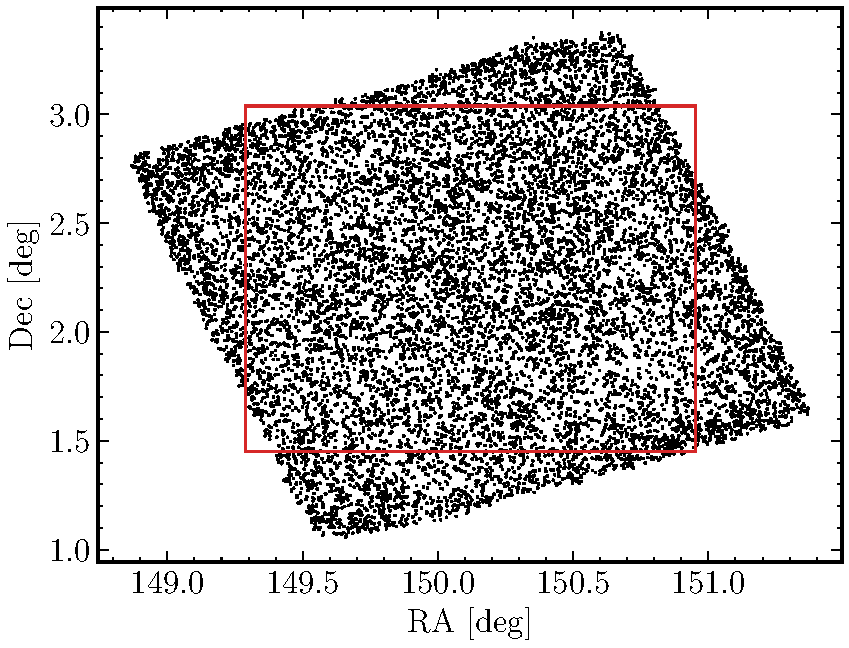
\includegraphics[width=0.75\columnwidth]{Figures/sky_map.pdf}
	\caption{{\color{red} Caption.}}
	\label{fig:sky_map}
\end{figure}

\subsection{The COSMOS2020 Catalogue}

{\color{red}Description of the COSMOS2020 catalogue.}

\subsection{Calculating the Significance of Associations}

To predict the probability that a sub-mm-radio pair is a significant association we could use the corrected Poisson probability defined by \citealt{Downes_1986}. This measures the Poisson probability that a radio source of a given flux density could lie at the observed distance from the source by chance. In this original paper the Poisson probability is defined as $P = 1-e^{-\mu}$ where $\mu = \pi r^2n$. Here $r$ is the radial offset between the source and radio counterpart and $n$ is the surface density of objects brighter than the radio counterpart. While a low value of $P$ does not confirm that the radio source is the correct ID for the sub-mm source, it suggests that the two are likely associated. A low value of $P$ can be interpreted in a number of ways. First, the radio source could be the true counterpart of the sub-mm source. Second, the counterpart could be one of a group of galaxies that collectively contribute to the flux density observed in the sub-mm. This is a very plausible case for the sources in our sample given the large beam sizes for \textit{Herschel}-SPIRE. Third, the low value of $P$ could be the result of an indirect association with the source, for example, due to clustering with the true ID or from the effects of gravitational lensing (although in the case of gravitational lensing this seems unlikely for our sample, as this would suggest that the lenses are as dust obscured as the background sources).

We used the method of \citealt{Lilly_1999} which applies the principles of the Poisson probability from \citealt{Downes_1986} in a Monte Carlo approach. The method, which is given in detail in \citealt{Dye_2009}, is as follows. First, we generate a set of $N$ random positions in the area common to both the sub-mm and radio surveys. Next, we identify all radio sources within some maximum radius, $r_{\textrm{max}}$, from each random position. For each radio source we measure the quantity $S = r^2n$, where $r$ and $n$ take the same definitions as earlier. The minimum value of $S$ for each source (corresponding to the most significant association in the case where multiple radio sources are observed) is retained. This defines our distribution, $D(S)$, which represents the distribution of $S$ values for random chance alignments. This distribution allows us to determine the probability of an observed radio source with $S = S_i$ and within $r_{\textrm{max}}$ of a sub-mm source being a random interloper. This is computed as:

\begin{equation}
    P(< S_i) = \frac{1}{N}\int_0^{S_i}D(S) dS.
    \label{eq:probability_frequentist}
\end{equation}

As is often assumed, we consider a radio source to be a secure identification if it has $P < 0.05$, suggesting that there is less than a 5\% probability that such a radio source would be observed by chance (e.g. \citealt{Ivison_2002}; \citealt{Ivison_2005}; \citealt{Pope_2006}). Depending on the surface density of radio galaxies, the maximum value of $P$ will often be less than one as some fraction of the randomly chosen positions will not contain any radio sources within $r_{\textrm{max}}$. 

The value of $r_{\textrm{max}}$ is an important choice. While a smaller search radius reduces the number of potential IDs and increases the likelihood of missing a true counterpart, a larger radius causes a greater probability of observing a background object and thus matching the source with an unrelated radio galaxy. A further problem is that too large a search radius causes overlapping fields which could lead to radio sources being connected to more than one sub-mm position. Previous studies (e.g. \citealt{Dye_2009}) have defined the maximum radius using a probabilistic balance between these two competing effects, finding the radius where the expected number of false counterparts in the final sample equals the expected number of true counterparts that are excluded. In this study we are attempting to define a clean sample of radio matched \textit{Herschel} sources, such that our multiwavelength counterparts from the COSMOS field represent a near complete and thorough description of the optical to radio properties of \textit{Herschel} detected sources. As we shall show later, this sample could provide a useful starting point for identifying dusty galaxies in future large area surveys (e.g. \textit{Euclid}) given that our sample will define some subpopulation of the COSMOS survey. For this reason, we are less interested in retaining the appropriate size of the sample, but rather in minimizing the number of falsely identified counterparts that would obfuscate our picture of dusty galaxies. 

Figure \ref{fig:optimal_radius} shows the radial distribution of VLA sources from the 7,230 \textit{Herschel} positions. Also shown is the number of matches with 7,230 random positions. The peak at small separations illustrates the excess of true counterparts over the background level. At larger separations the number of matches with \textit{Herschel} positions follows the linear relation observed around random positions. The number of VLA sources observed at $r \sim 10$\,arcsec from \textit{Herschel} positions and random positions is approximately equal, corresponding to the radial offset beyond which we expect the probability of a counterpart being associated with the source is dominated by chance alignments. This radius may seem prone to misidentification, but if we consider the cumulative number of counterparts to a search radius $r$ (inset figure), then we see that a maximum search radius of $r_{\textrm{max}} \approx 10$\,arcsec corresponds to a maximum in the excess of expected true counterparts over background sources. This implies that at this radius the number of counterparts observed within the search radius is dominated by true counterparts, which will aid in reducing the false identification rate.

\begin{figure}
	\centering
	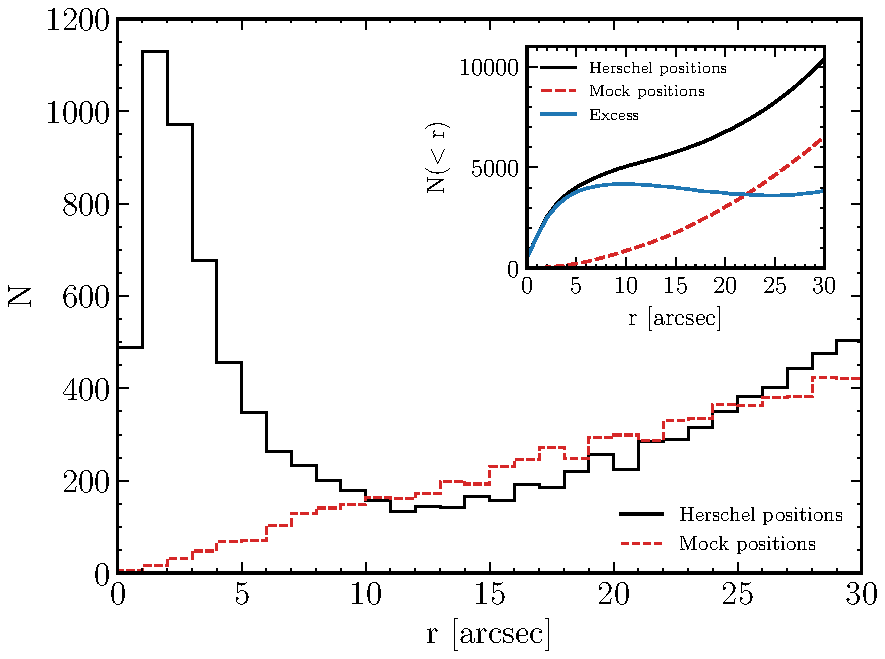
\includegraphics[width=0.75\columnwidth]{Figures/optimal_radius.pdf}
	\caption{{\color{red} Caption.}}
	\label{fig:optimal_radius}
\end{figure}

Given that our VLA observations have a surface density of $4103\,$deg$^{-2}$ and we are assuming a maximum search radius of 10\,arcsec, we can approximate the maximum value of $P$. As a first order approximation, the maximum $P$ value is equal to the ratio between the probability of observing at least one VLA source within the search radius of a random position and the probability that the position is a blank field. Assuming Poisson statistics with a mean number of counterparts per random position of $\lambda = N_{\textrm{VLA}}A_{\textrm{random}}/A_{\textrm{survey}}$, where $N_{\textrm{VLA}}$ is the number of VLA sources, $A_{\textrm{random}}$ is the search area around a random position and $A_{\textrm{survey}}$ is the total survey area, then an estimate of $P_{\textrm{max}}$ can be given by:

\begin{equation}
    P_{\textrm{max}} \approx \frac{P(\textrm{Not Blank})}{P(\textrm{Blank})} = \frac{P(X > 0)}{P(X = 0)} = \frac{1 - P(X = 0)}{P(X = 0)} = \frac{1 - e^{-\lambda}}{e^{-\lambda}} \approx 0.10,
\end{equation}

\noindent where $X$ is the number of VLA sources observed around each random position. This calculation suggests that the maximum $P$ value for any radio source observed near a \textit{Herschel} source is $0.1$, not considering effects such as clustering, multicomponent galaxies or overlapping search areas. The fact that only $\sim$ 10\% of random positions will be incident with at least one radio source gives further confidence in the association between any \textit{Herschel} and VLA sources in close proximity.

\section{Results of the Frequentist Method Applied to \textit{Herschel} Sources}

We apply the method described above to all possible VLA counterparts within 10 arcsec of a SPIRE source. We retain all counterparts that have $P < 0.05$, but consider as our primary counterparts those with the lowest $P$ value per \textit{Herschel} source. Figure \ref{fig:ds_distributions} shows the distribution of $S$ for radio counterparts to \textit{Herschel} (black histogram) and $10^6$ random positions (red histogram). The clear offset between the two distributions illustrates how a large fraction of the counterparts identified in the radio trace the sub-mm sources.

\begin{figure}
	\centering
	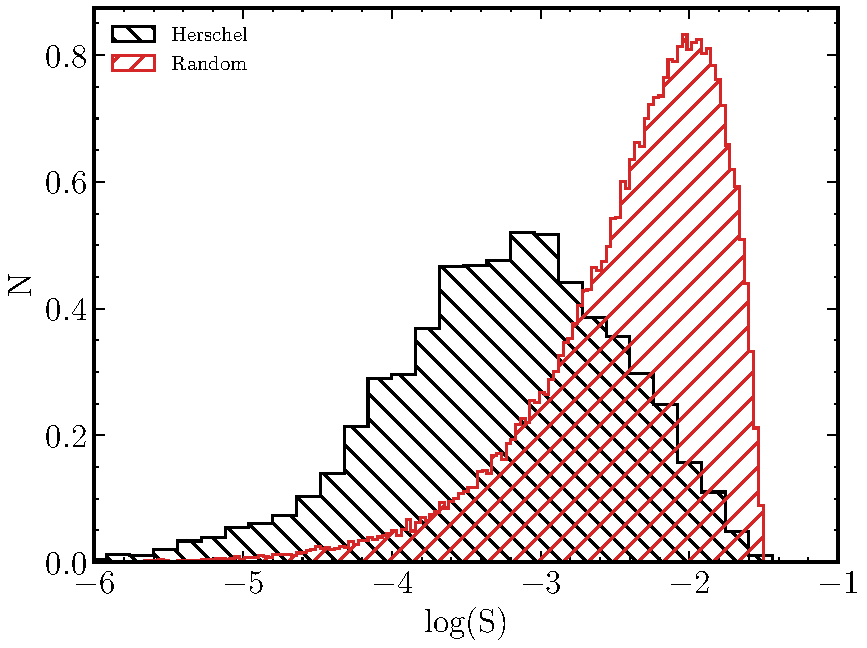
\includegraphics[width=0.75\columnwidth]{Figures/ds_distributions.pdf}
	\caption{{\color{red} Caption.}}
	\label{fig:ds_distributions}
\end{figure}

The total identification rate, that is the number of sources identified with $P < 0.05$ by a radio source, is 3,787/7,230 (52\%). However, the identification rate is a strong function of the sub-mm flux density (Figure \ref{fig:id_rate}). There is a strong decline toward fainter 250\,\micron\ fluxes ($< 30\,$mJy) where we approach the confusion limit of the survey. To be consistent with our motivation for a clean and unambiguous sample of \textit{Herschel} galaxies and their multiwavelength properties, we henceforth refer only to the sources with 250\,\micron\ flux densities greater than 30\,mJy, where we are more confident that they correspond to true sources. The survey area corresponds to 1,324 \textit{Herschel} sources with $S_{250\,\mu m} > 30\,$mJy. Of these sources, 1,053 (80\%) have radio IDs with $P < 0.05$. {\color{red}Some comment about it being 80\% - much better than optical/near-IR LR. Why?}

\begin{figure}
	\centering
	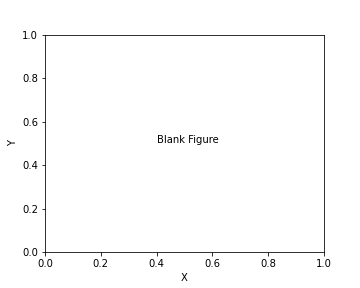
\includegraphics[width=0.75\columnwidth]{Figures/blank_figure.png}
	\caption{{\color{red} Caption.}}
	\label{fig:id_rate}
\end{figure}

Given that $P_i$ represents the probability of observing a radio counterpart, $i$, with a given flux and offset from the source by chance, the number of false IDs in a $P$-limited sample is given by

\begin{equation}
    N_{\textrm{False}} = \sum_{P_i < 0.05} P_i,
    \label{eq:false_radio_ids}
\end{equation}

\noindent which is analogous to Equation \ref{eq:false_ids} when using the LR method. 
